% !TeX spellcheck = it_IT
\newpage
\section{UML}
Unified Modelling Language è un linguaggio di modellazione che supporta la descrizione e la progettazione di progetti software (in particolare OO). Descrive da un punto di vista \textbf{strutturale} e \textbf{comportamentale}, del dominio e del codice, della progettazione e della fase finale.\\
Utilizza \textbf{famiglie grafiche} che comprendono diversi punti di vista, sono correlate e facilmente interpretabili.
\subsection{Modello}
Un modello è un'\textbf{astrazione} a partire dai dettagli, del sistema o dominio usato per specificarne il \textit{comportamento} e la \textit{struttura}.  È espresso con un formalismo ed è descritto da un insieme di \textbf{viste}.\\
È uno strumento di documentazione, comunicazione e discussione fondamentale per un progetto di sviluppo software.

\subsubsection{Modellazione}
Un modello può essere:
\begin{itemize}
	\item \textbf{Statico}: vengono usate \textbf{entità} e \textbf{relazioni} per descrivere tutti gli aspetti indipendenti dal tempo:
	\begin{itemize}
		\item Concetti del \textit{dominio}
		\item Componenti dell'\textit{architettura}
		\item Classi di \textit{realizzazione}
	\end{itemize}
	\item \textbf{Dinamico}: modella il comportamento delle entità descritte in quello statico
\end{itemize} In questa fase si decide anche il livello di astrazione.
\subsubsection{Rappresentazione}
Si rappresenta con un linguaggio formale o semi formale.
\subsubsection{Utilizzo}
A seconda del livello del modello, ha scopi diversi:
\begin{itemize}
	\item \textbf{Sketch}: non completo, usato per le descrizioni iniziali
	\item \textbf{Blueprint}: sufficiente a creare un sistema capace di funzionare
	\item \textbf{Eseguibile}: talmente completo e preciso da generare automaticamente il codice
\end{itemize}

\subsection{Storia}

\begin{center}
	\begin{tikzpicture}
		\draw (0,0) -- (15.5,0);
		
		\foreach \x in {1,3.5,6,10, 14}
		\draw (\x cm,-0.1) -- (\x cm,0.1);
		
		\draw (1,0) node[below=3pt] {prima 1994} node[above=3pt] {\parbox{10em}{\centering Molti linguaggi e \\ metodi diversi}};
		\draw (3.5,0) node[below=3pt] {1994} node[above=3pt] {\textbf{Fusion}};
		\draw (6,0) node[below=3pt] {1994} node[above=3pt] {\parbox{10em}{\centering Booch e Rumbaugh \\ propongono \textbf{UML}}};
		\draw (10,0) node[below=3pt] {1996} node[above=3pt] {\parbox{15em}{\centering Object Management Group \\ propone uno standard}};
		\draw (14,0) node[below=3pt] {1997} node[above=3pt] {\parbox{15em}{\centering OMG approva\\ \textbf{UML 1.0}}};
		
		\draw (15.5,0) -- (15.5,-2);
		
		\draw [-{Latex[length=3mm, width=2mm]}](15.5,-2) -- (0,-2);		
		
		\foreach \x in {3,8,13}
		\draw (\x cm,-2.1) -- (\x cm,-1.9);
		
		\draw (13,-2) node[above=3pt] {2000} node[below=3pt] {\textbf{UML 1.4}};
		\draw (8,-2) node[above=3pt] {2006} node[below=3pt] {\textbf{UML 2.0}};
		\draw (3,-2) node[above=3pt] {2006} node[below=3pt] {\textbf{Model Driven Architecture}};
	\end{tikzpicture}
\end{center}

\subsection{Diagrammi}
\subsubsection{Casi d'uso}
Questo diagramma modella i requisiti del sistema: raccoglie quelli \textit{funzionali}, li elabora e li documenta. Il modello statico è il diagramma dei casi mentre quello dinamico contiene le narrative a loro associate.
\begin{definition}[Attore]
	Un attore è un'\textbf{entità estranea} al sistema che \textbf{interagisce} direttamente con esso in un determinato \textbf{ruolo}. Può essere di tre tipi:
	\begin{itemize}
		\item Utente \textbf{umano} in un determinato \textbf{ruolo}
		\item Un \textbf{sistema} differente
		\item \textbf{Tempo}
	\end{itemize}
\end{definition}

\begin{definition}[Caso d'uso]
	Un caso d'uso è un \textbf{compito} che un \textbf{attore} può svolgere con l'aiuto del sistema. Viene espresso come insieme di scenari.
\end{definition}

\begin{definition}[Scenario]
	Uno scenario è una sequenza di \textbf{interazioni} tra sistema e attori. Viene espresso come scambio di messaggi.
\end{definition}

\noindent La modellazione di questo tipo di diagramma si divide nelle seguenti fasi:
\begin{enumerate}
	\item Individuare il \textbf{confine} del sistema
	\item Individuare gli \textbf{attori}
	\item Individuare i \textbf{casi d'uso}
	\item Individuare le \textbf{relazioni} tra attori e casi d'uso
	\item Specificare il caso d'uso con una \textbf{narrativa}
\end{enumerate}

\paragraph{Notazione} In questo tipo di diagramma abbiamo \textit{attori} e \textit{casi d'uso} indicati con la lettera maiuscola. Le \textit{relazioni} che rappresentano lo scambio di messaggi sono linee e il \textit{confine del sistema} è un rettangolo intorno ai casi d'uso.
\begin{center}
	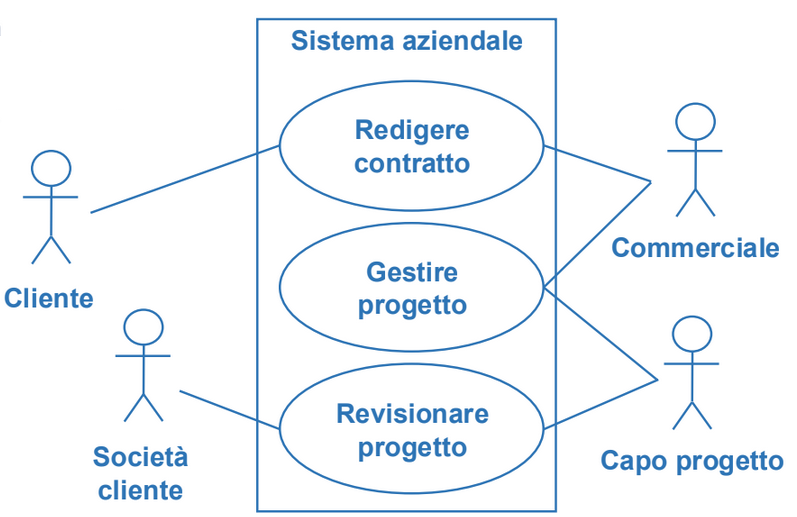
\includegraphics[scale=0.3]{uml_casiuso.png}
\end{center}

\begin{note}
	L'associazione tra attori e casi d'uso è di tipo \textbf{molti a molti} in quanto un attore può essere associato a più casi e un caso a più attori.
\end{note}

\begin{note}
	Un caso può essere \textbf{iniziato} solamente da uno ed un solo attore, detto \textbf{principale} (che può essere il Tempo). Ci sono casi specifici in cui non ci sono attori.
\end{note}

\newpage
\paragraph{Narrativa}
La narrativa descrive il modello dinamico, ovvero gli \textbf{scenari} rilevanti per un caso d'uso dal punto di vista degli attori, compreso il principale. La \textbf{struttura} è la seguente:
\begin{table}[!h]
	\centering
	\begin{tabular}{|c|c|}
		\hline
		\textbf{Nome} & Nome del caso d'uso\\
		\hline
		\textbf{ID} & Identificatore univoco del caso \\
		\hline
		\textbf{Breve descrizione} & $\ldots$\\
		\hline
		\textbf{Attore primario} & Colui che avvia il caso \\
		\hline
		\textbf{Attori secondari} & Tutti gli attori che interagiscono \\
		\hline
		\textbf{Precondizioni} & Ciò che deve valere prima dell'esecuzione\\
		\hline
		\textbf{Sequenza degli eventi principale} & Sequenza di passi \\
		\hline
		\textbf{Postcondizioni} & Ciò che deve valere dopo l'esecuzione \\
		\hline
		\textbf{Sequenze alternative degli eventi} & Errori, ramificazioni e interruzioni\\
		\hline
	\end{tabular}
\end{table}

\paragraph{Scenario}
Uno scenario è un'\textbf{istanza} di un caso d'uso, quindi una sequenza di passi che produce un risultato osservabile da uno o più attori. Portano dalla \textit{precondizione} alla \textit{postcondizione}.
\begin{center}
	
\includegraphics[scale=0.3]{uml_casiuso_scenari.png}
\end{center}

\begin{definition}[Pre e post condizioni]
	Precondizioni e postcondizioni sono \textbf{asserzioni} che devono necessariamente essere vere in uno stato. Si esprimono con \textbf{predicati} e \textbf{formule logiche}. \color{red} Non sono MAI azioni. \color{black}
\end{definition}

\begin{definition}[Flusso di narrativa]
	Per ogni stato $\sigma$ che soddisfa la \textbf{precondizione}, l'esecuzione del caso d'uso a partire da $\sigma$ produce uno stato $\sigma '$ che soddisfa la \textbf{postcondizione}. Questo a meno di imprevisti elencati nella \textit{sequenza alternativa}.
\end{definition}

\paragraph{Sequenza principale}
Indica la sequenza di passi che compongono il caso d'uso. È \textbf{numerata} e ogni passo ha la struttura
\begin{equation*}
	<\text{numero}>.<\text{soggetto}><\text{azione}><\text{complementi}>
\end{equation*}
Il primo passo è detto \textbf{attivazione} ed è compiuto sempre dall'attore principale.

\paragraph{Generalizzazione} È possibile generalizzare gli \textbf{attori}, ad esempio quando c'è bisogno di un unico attore principale (e.g. \textit{professore} e \textit{assistente} sono \textit{ricercatori}), o i \textbf{casi d'uso} (e.g. \textit{card} e \textit{cash} sono \textit{pagamenti}). Bisogna prestare attenzione perché il classificatore specializzato \textbf{eredita} tutte le relazioni di quello padre a meno che non sia esplicitato il contrario.

\begin{definition}[Stereotipo]
	Gli stereotipi sono parole chiave racchiuse tra $<<>>$ che annotano gli elementi di un diagramma, precisandone il significato.
\end{definition}

\paragraph{Inclusione} Un caso d'uso può incorporarne un altro tramite l'\textbf{inclusione}, ovvero la chiamata del primo ha come conseguenza la chiamata del secondo.
\begin{center}
	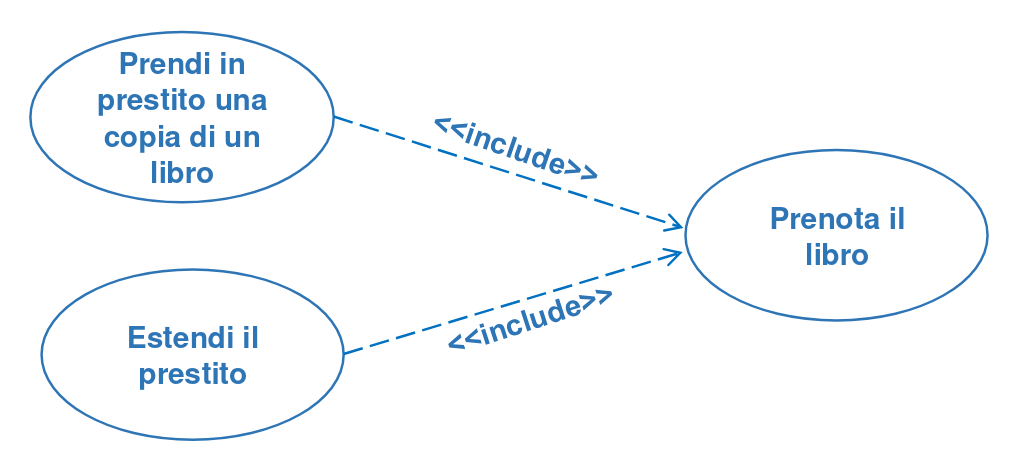
\includegraphics[scale=0.2]{inclusione.png}
\end{center}
Nella narrativa l'inclusione può avvenire in maniera \textit{istanziabile} quando viene avviato da un attore primario o \textit{non istanziabile} quando viene eseguito solo dopo l'inclusione da parte di un altro caso.

\paragraph{Estensione} Quando il primo caso d'uso \textit{può} prevederne un altro, si dice che lo incorpora. Di conseguenza le estensioni sono opzionali e per specificare quando si presentano è possibile usare un \textbf{extension point} con all'interno la condizione che si deve verificare.
\begin{center}
	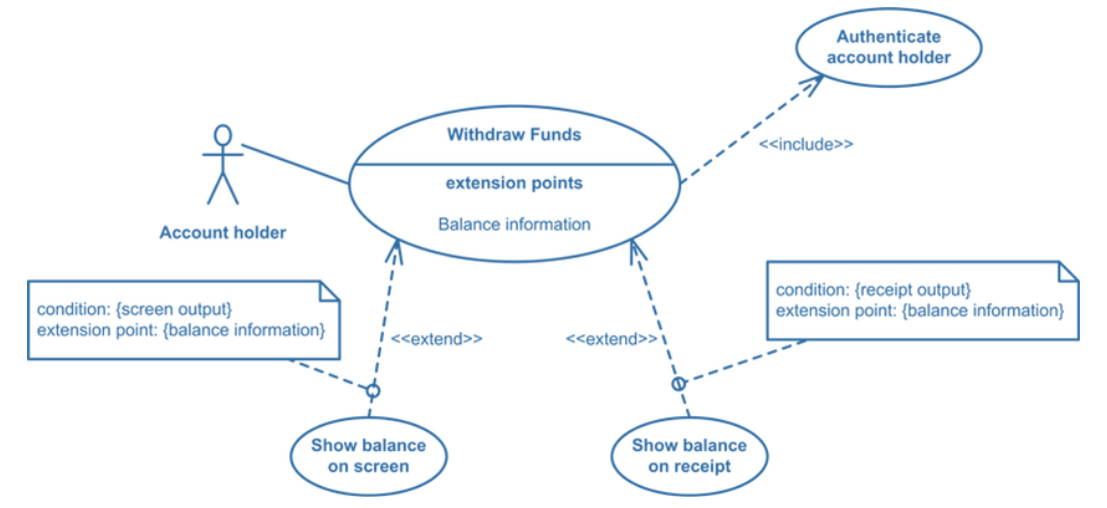
\includegraphics[scale=0.3]{extension.png}
\end{center}

\subsubsection{Classi e oggetti}
Il diagramma delle classi descrive il tipo degli oggetti che fanno parte di un sistema e le relazioni statiche tra di esse. Mostra inoltre le \textbf{proprietà} e le \textbf{operazioni} delle classi. Può essere utilizzato per descrivere il \textit{dominio} o per fare una \textit{progettazione} di dettaglio. 

\begin{definition}[Oggetto]
	Un oggetto è un'identità caratterizzata da un'\textbf{identità}, uno \textbf{stato} (valori e rispettivi attributi) e un \textbf{comportamento} (operazioni che lo definiscono).
\end{definition}
\begin{definition}[Classe]
	Una classe descrive un insieme di oggetti con caratteristiche simili, ovvero dello stesso tipo. Cattura un \textbf{concetto} nel dominio del problema o della realizzazione.
\end{definition}
\noindent In UML la classe contiene:
\begin{itemize}
	\item \textbf{Nome}: maiuscolo singolare
	\item \textbf{Attributi} tipizzati con modificatori di visibilità:
	\begin{itemize}
		\item \textit{Pubblic} \textbf{+} : accessibile ad ogni elemento che può vedere e usare la classe
		\item \textit{Protected} \textbf{\#} : accessibile ad ogni discendente
		\item \textit{Private} \textbf{-} : solo le operazioni della classe vi hanno accesso
		\item \textit{Package} \textbf{\texttildelow} : solo gli elementi dello stesso \textit{package} vi hanno accesso
	\end{itemize}
	\item \textbf{Operazioni} tipizzate
\end{itemize}
\paragraph{Attributi}
La sintassi degli attributi è la seguente:
\begin{equation*}
	\text{visibilità } \textcolor{blue}{nome}: \text{tipo}[\text{\textcolor{orange}{molteplicità}}] = \text{ \textcolor{gray}{valoreIniziale} } \{\text{\textcolor{green}{proprietà}}\}
\end{equation*}
\begin{note}
	La molteplicità $[1]$ può essere omessa.
\end{note}
Degli esempi di \textbf{proprietà} sono \textit{ordered}, \textit{unique} o vincoli in generale (e.g. $\{>0, <10\}$).

\begin{note}
	Quando viene usato per la definizione del dominio, si omettono generalmente \textit{operazioni} e \textit{modificatori di visibilità} e si inseriscono solo gli \textit{attributi} utili ad esso.
\end{note}

\paragraph{Operazioni}
La sintassi delle operazioni è la seguente:
\begin{equation*}
	\text{visibilità } \textcolor{blue}{nome(} \text{\textcolor{orange}{lista parametri}}\textcolor{blue}{)}: \text{tipoRitorno}
\end{equation*}
Dove la lista dei parametri può essere l'\textbf{insieme vuoto} o una \textbf{dichiarazione} di parametro:
\begin{align*}
	\text{\textcolor{orange}{lista parametri}} ::= \emptyset \quad \vert \quad \text{dichiarazione} \\
	\text{dichiarazione} ::= \text{\textcolor{green}{nome}} : \text{tipo} = \text{\textcolor{gray}{default}}
\end{align*}

\begin{note}
	L'unica parte obbligatoria della sintassi è il \textbf{nome}, sia nelle operazioni che in \textit{eventuali} parametri.
\end{note}

\begin{note}
	Attributi e operazioni \textbf{statici}, quindi con ambito di classe, sono \underline{sottolineati}.
\end{note}

\paragraph{Enumerazioni} Le enumerazioni sono usate per specificare un insieme di valori \textbf{prefissati} ovvero tutti i valori che un attributo può assumere.\\
In UML hanno sono \textit{classi} con un nome (il tipo) e l'elenco dei valori. Sono etichettate dallo \textit{stereotipo}
\begin{equation*}
	<<\text{enumeration}>>
\end{equation*}

\subsubsection{Relazioni}
Una relazione rappresenta un legame tra due o più oggetti, di solito istanze di classi diverse.

\begin{table}[!h]
	\centering
	\begin{tabular}{|c|c|}
		\hline
		\textbf{Tra classificatori} & \textbf{Tra oggetti}\\
		\hline
		Associazione & Collegamento \\
		\hline
		Generalizzazione & \textit{(non definita)} \\
		\hline
		Realizzazione & \textit{(non definita)} \\
		\hline
		\multicolumn{2}{|c|}{Dipendenza (d'uso, d'istanza, etc..)}\\
		\hline
	\end{tabular}
\end{table}
\paragraph{Associazione}
Un'associazione è una linea retta con:
\begin{itemize}
	\item \textbf{Nome}, di solito un verbo
	\item \textbf{Ruoli}, di solito sostantivi
	\item \textbf{Verso} di lettura, opzionale
\end{itemize}
Di solito si usa o il \textit{nome} o i \textit{ruoli}, raramente entrambi. \\
È importante anche specificare i \textbf{vincoli di molteplicità}, ovvero il numero di oggetti coinvolti nell'associazione in un dato istante. Si possono definire:
\begin{itemize}
	\item Con un \textbf{numero positivo}
	\item Con il \textbf{simbolo indefinito} (*), ovvero per un qualunque numero $\geq 0$
	\item Indicando gli \textbf{estremi dell'intervallo}, dove quello \textit{inferiore} può essere $\geq 0$ e quello superiore un numero positivo o il simbolo indefinito
\end{itemize}
\begin{example}
	Esempio di molteplicità:
	\begin{center}
		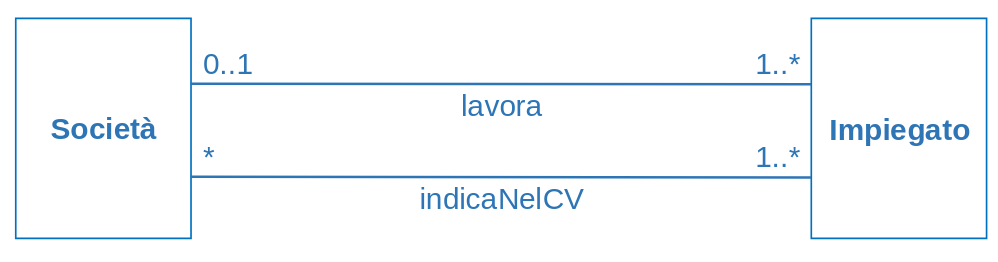
\includegraphics[scale=0.3]{molteplicita.png}
	\end{center}
\end{example}
Un associazione può mettere in relazione un'entità con se stessa, in questo caso è detta \textbf{riflessiva}.\\
Esistono due tipi specifici di associazioni che vengono utilizzati per specificare se un oggetto fa parte o meno di un'altra classe:
\begin{itemize}
	\item \textbf{Aggregazione} ($\Diamond$), poco forte, usata quando la classe "parte" esiste anche senza quella "tutto"
	\item \textbf{Composizione} ($\mathbin{\blacklozenge}$), molto forte, usata quando la classe "parte" non esisterebbe senza quella "tutto". Non ha un nome.
\end{itemize}
\begin{example}
	Esempio di aggregazione e composizione:
	\begin{center}
		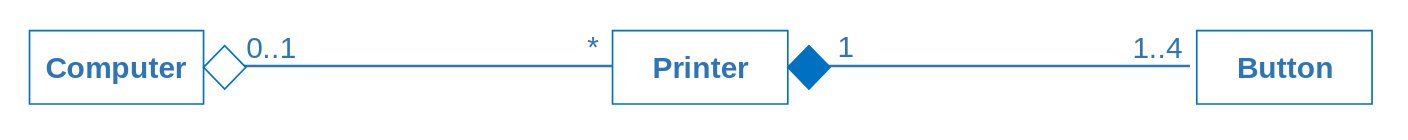
\includegraphics[scale=0.3]{aggr_comp.png}
	\end{center}
\end{example}

\paragraph{Generalizzazione}
È una relazione tra un elemento generico $G$ e uno specializzato $S$, che è consistente con il primo ma contiene più informazione. Per il \textit{principio di sostituzione di Liskov} $S$ può essere sostituito con $G$.
\begin{center}
	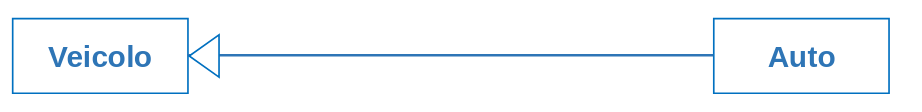
\includegraphics[scale=0.3]{generaliz.png}
\end{center}
Una \textit{superclasse} generalizza le sottoclassi e queste \textbf{ereditano} \textit{attributi}, \textit{operazioni}, \textit{relazioni} e \textit{vincoli}. La sottoclasse può aggiungere caratteristiche e ridefinire determinate operazioni.
\begin{center}
	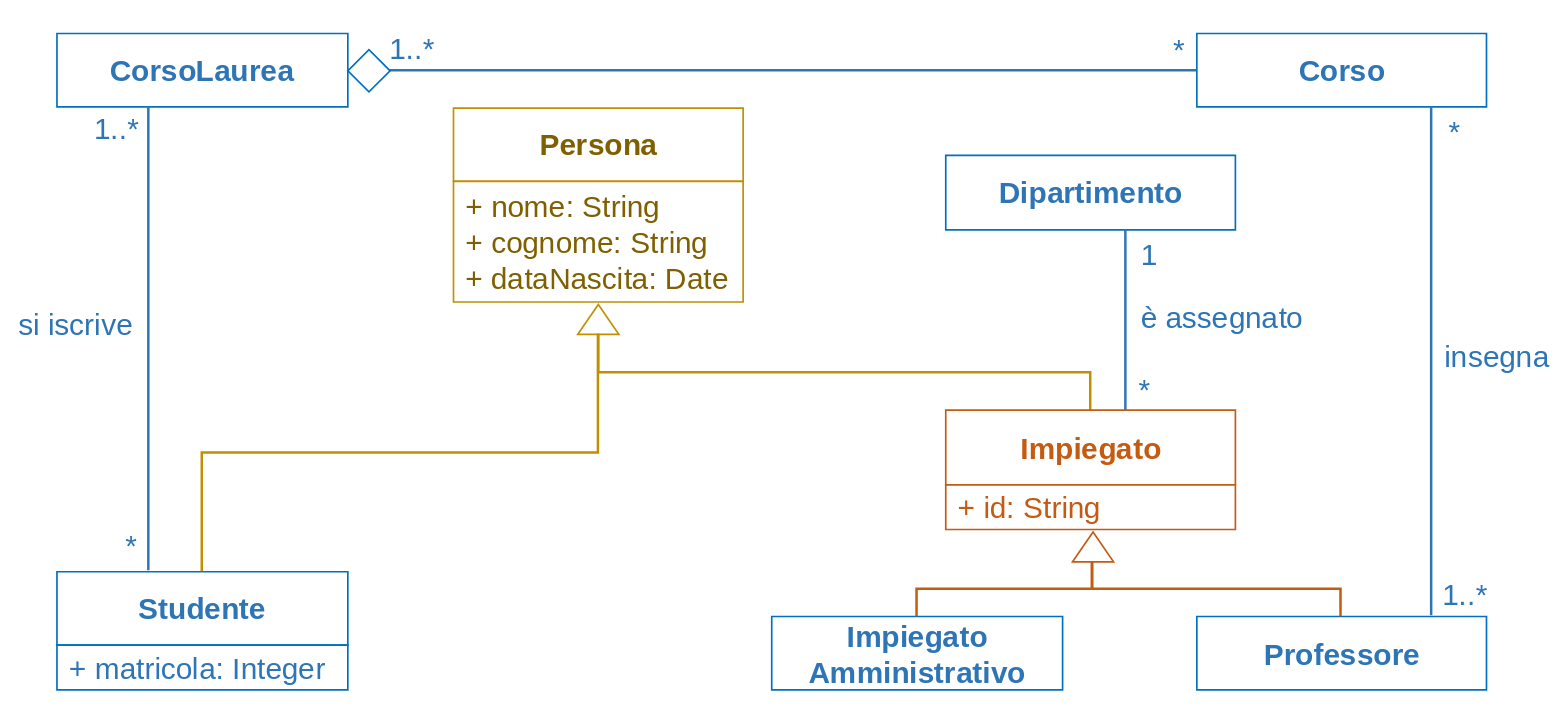
\includegraphics[scale=0.25]{generaliz_ex.png}
\end{center}

\begin{definition}[Classe astratta]
	Nell'ambito della generalizzazione, quando una classe esiste puramente per essere poi estesa e specializzata, viene definita \textbf{astratta}. In questo caso o si usa il nome in corsivo o si indica 
	\begin{equation*}
		\{\text{abstract}\}
	\end{equation*}
\end{definition}

\begin{definition}[Interfaccia]
	Un'interfaccia è un'entità che contiene solamente il comportamento ma nessuno stato. Viene indicata dallo stereotipo
	\begin{equation*}
		<<\text{interface}>>
	\end{equation*}
\end{definition}

\paragraph{Dipendenza}
Una dipendenza è una relazione tra una classe \textbf{cliente} e una \textbf{fornitore}, dove il primo dipende dal secondo e una modifica nel secondo influenza il primo. Viene indicata da una linea tratteggiata con uno dei seguenti stereotipi a seconda del caso
\begin{equation*}
	<<\text{use}>> \qquad <<\text{create}>>
\end{equation*}

\subsubsection{Classi di analisi}
Le classi di analisi corrispondo a concetti concreti del \textit{dominio}, e.g. il contenuto del glossario. Viene spesso raffinata in una o più classi di \textit{progettazione}. Il loro compito è quello di \textbf{astrarre} un elemento del dominio. Generalmente devono seguire le seguenti caratteristiche:
\begin{itemize}
	\item Numero ridotto di funzionalità
	\item Evitare classi \textit{onnipotenti}
	\item Evitare funzioni travestite da classi
	\item Evitare gerarchie di ereditarietà $\geq 3$
\end{itemize}
Esistono principalmente due approcci per identificare le classi di analisi:
\begin{itemize}
	\item \textbf{Data-driven}: si identificano i dati del sistema e si dividono in classi, tipico per la fase di analisi
	\item \textbf{Responsibility-driven}: si identificano le responsabilità e si dividono in classi, tipico per la fase di progettazione
\end{itemize}
\paragraph{Analisi nome-verbo}
Una tecnica per eseguire l'identificazione dove ogni \textbf{sostantivo} corrisponde ad una \textit{classe} o \textit{attributo} mentre ogni \textbf{verbo} ad un'operazione.\\
Consiste in:
\begin{enumerate}
	\item Individuazione delle classi
	\item Assegnazione di attributi e responsabilità
	\item Individuazione delle relazioni
\end{enumerate}
Le problematiche principali sono i sinonimi che portano a classi \textbf{inutili} e le classi \textbf{nascoste} perché implicite nel dominio.

\subsubsection{Diagramma degli oggetti}
Un oggetto si rappresenta con il \textbf{nome}, la \textbf{classe} che istanzia, \underline{sottolineati} e la lista degli \textbf{attributi} (nome, tipo e valore).
\paragraph{Collegamento} Un collegamento istanzia un'associazione nel diagramma delle classi collegando due o più oggetti. Non ha nome, ha sempre molteplicità $1:1$ e può includere i ruoli

\begin{figure}[!h]
	\centering
	\begin{minipage}[b]{0.5\textwidth}
		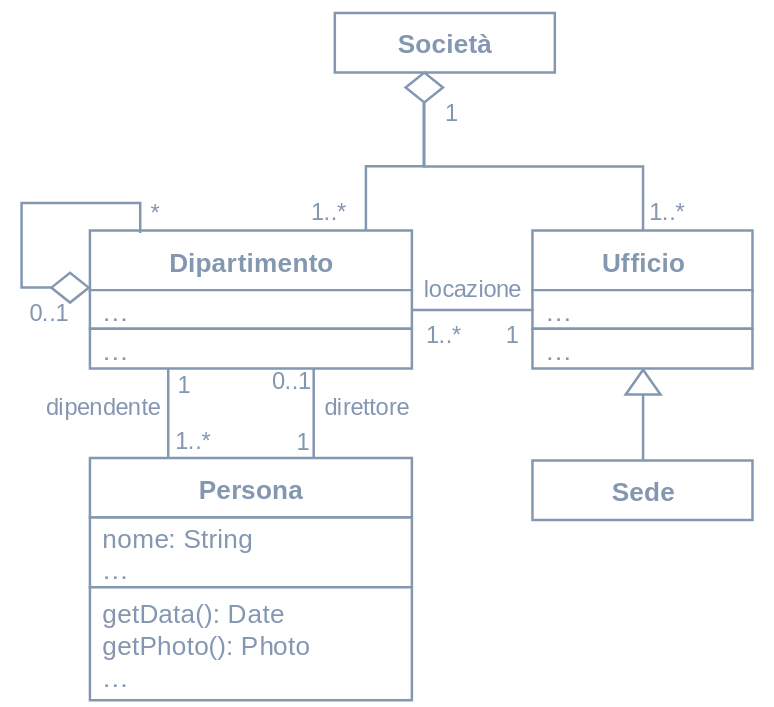
\includegraphics[width=\textwidth]{diag_class.png}
		\caption{Diagramma delle classi}
	\end{minipage}
	\hfill
	\begin{minipage}[b]{0.4\textwidth}
		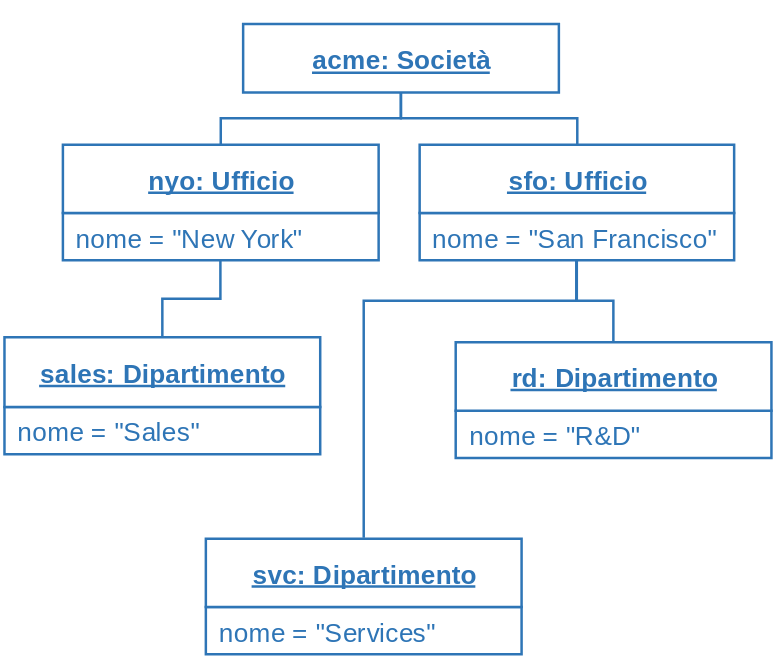
\includegraphics[width=\textwidth]{diag_obj.png}
		\caption{Diagramma degli oggetti}
	\end{minipage}
\end{figure}

\subsubsection{Diagramma delle attività}
Il diagramma delle attività modella un \textbf{workflow} e descrive come \textbf{coordinare} un insieme di \textbf{azioni}, quali \textit{sequenze}, \textit{scelte}, \textit{iterazioni} e \textit{concorrenza}.
Nello specifico modella un'attività in cui sono coinvolte una o più entità.\\
In UML è contenuta in un rettangolo dagli angoli smussati e ha un nome.
\begin{center}
	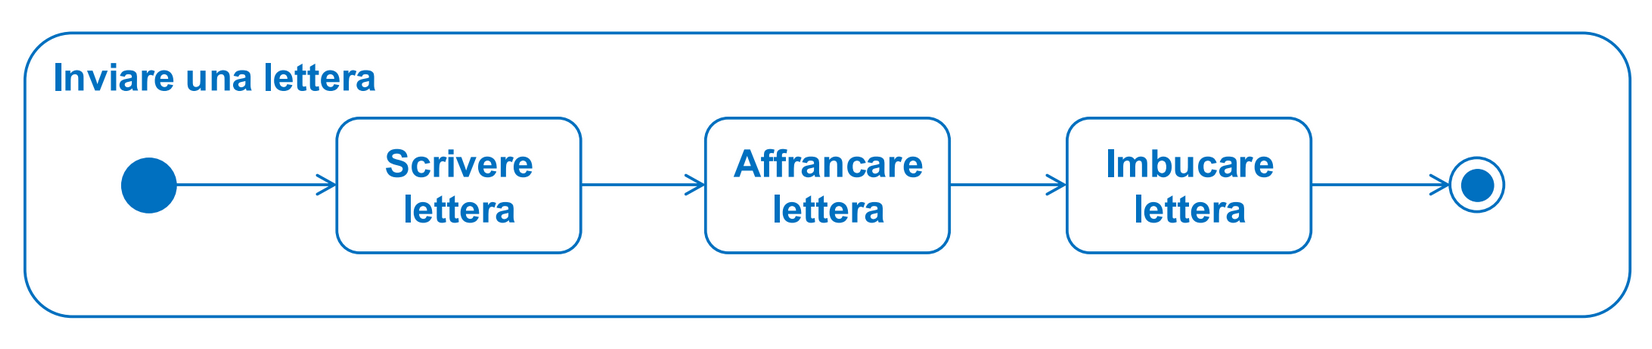
\includegraphics[scale=0.2]{activity.png}
\end{center}
Il contenuto dell'attività è un \textbf{grafo diretto}, dove i \textbf{nodi} rappresentano le componenti dell'attività (azioni e nodi di controllo quali inizio e fine) mentre gli \textbf{archi} rappresentano il \textbf{control flow}, ovvero i possibili path di esecuzione.

\paragraph{Azioni} Le azioni sono rettangoli con gli angoli smussati che contengono il nome che è sempre un \textbf{verbo}. Sono \textbf{atomiche} e non interrompibili.\\
Ogni azione ha solo un arco entrante ed uno uscente e quest'ultimo viene attraversato ad azione terminata, simulando il passaggio di un \textbf{token} che permette l'esecuzione.

\begin{note}
	I nomi delle azioni devono indicarne l'esecuzione e quindi dovrebbero essere verbi all'indicativo, imperativo o infinito oppure sostantivi che indichino un'azione.
\end{note}

\paragraph{Nodi di controllo} Sono nodi che alterano il control flow. Possono essere:
\begin{itemize}
	\item \textbf{Decisione} e \textbf{fusione}: sono rappresentati da rombi, nel primo caso con condizioni che devono coprire tutti i possibili casi ($X \lor Y \lor \ldots \lor Z = \text{true}$) e che portano a rami differenti. È possibile utilizzare la clausola \textit{$[\text{else}]$}. Non è obbligatorio che ci sia un nodo di fusione corrispondente.
	\begin{center}
		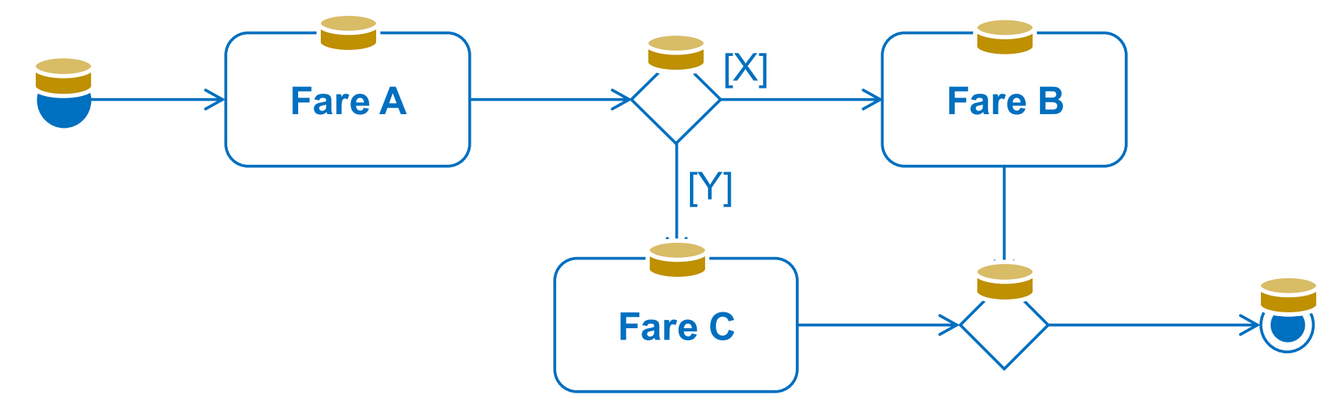
\includegraphics[scale=0.2]{decision_fusion.png}
	\end{center}
	\item \textbf{Fork} e \textbf{join}: la fork moltiplica i token e ne restituisce uno per ogni ramo uscente, al contrario la join (non ne serve per forza una per ogni fork), attende un token da ogni ramo, li consuma tutti e ne restituisce uno.
	\begin{center}
		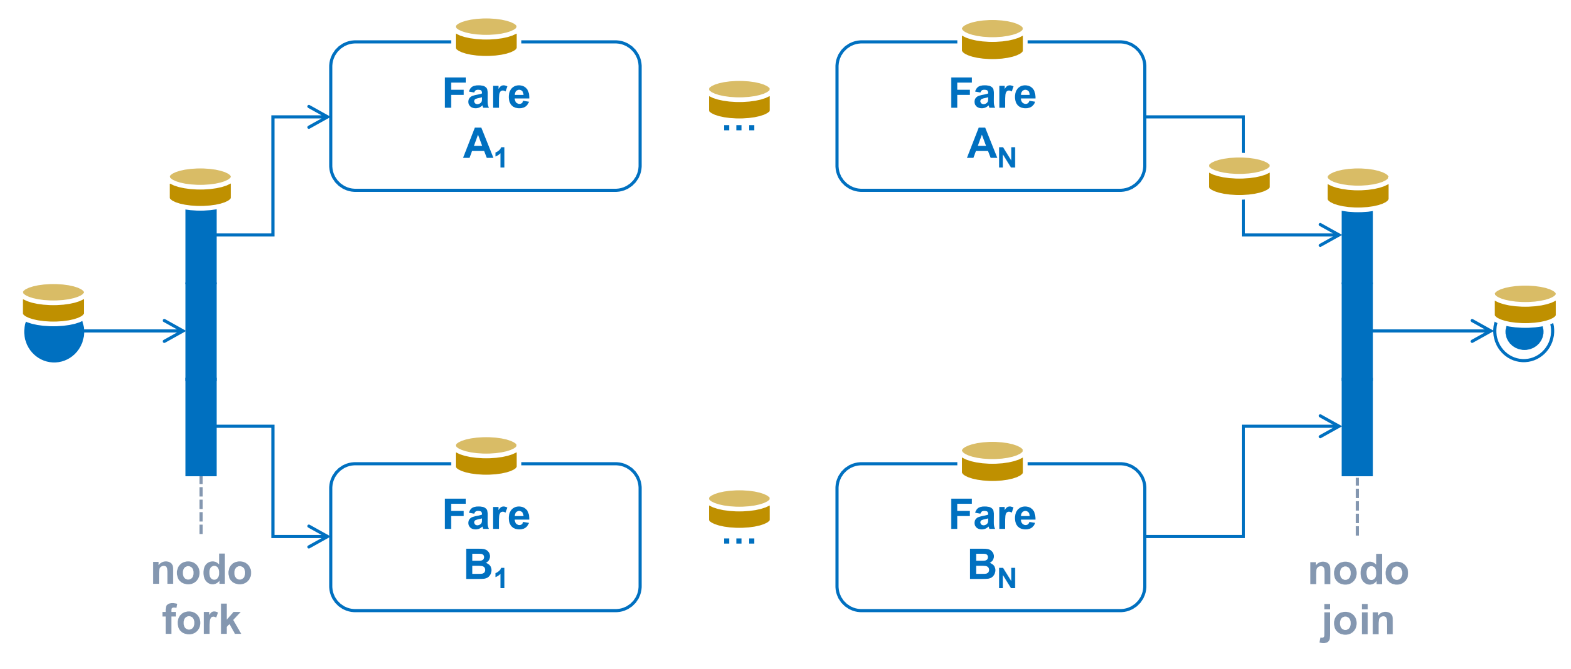
\includegraphics[scale=0.2]{fork_join.png}
	\end{center}
	\item \textbf{Fine attività} e \textbf{fine flusso}: gli unici nodi che possono avere più archi entranti. Il primo, appena riceve un token, termina l'intera attività mentre il secondo termina solo il flusso corrispondente.
	\begin{center}
		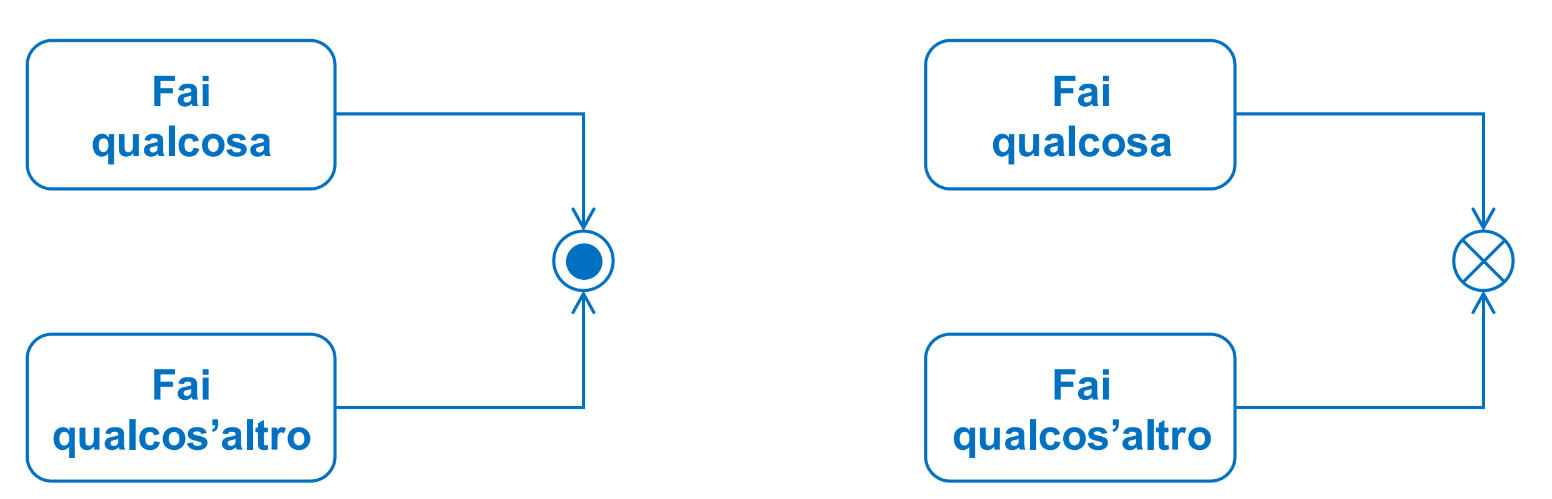
\includegraphics[scale=0.2]{end_node.png}
	\end{center}
	\newpage
	\item \textbf{Segnali} ed \textbf{eventi}: possono inviare un \textbf{segnale asincrono}, riceverlo o accettare un \textbf{evento temporale} (assoluto o relativo)
	\begin{figure}[!h]
		\centering
		\begin{minipage}[b]{0.2\textwidth}
			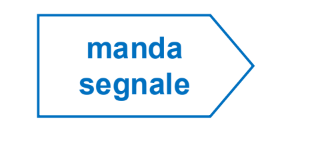
\includegraphics[width=\textwidth]{send_signal.png}
			\caption*{Invio}
		\end{minipage}
		\hspace{0.1\textwidth}
		\begin{minipage}[b]{0.2\textwidth}
			
\includegraphics[width=\textwidth]{accept_signal.png}
			\caption*{Accettazione}
		\end{minipage}
		\hspace{0.1\textwidth}
		\begin{minipage}[b]{0.2\textwidth}
			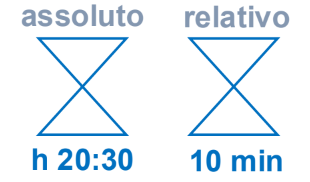
\includegraphics[width=\textwidth]{time_signal.png}
			\caption*{Evento temporale}
		\end{minipage}
	\end{figure}
	I nodi di accettazione non hanno bisogno di archi entranti: se non c'è si genera un token quando si verifica l'evento, altrimenti si attende prima di passarlo al nodo successivo.
\end{itemize}

\begin{note}[Fork e merge]
	È possibile eseguire una \textit{fork} e poi una \textit{merge} invece della join, ma questo vorrà dire che le operazioni dopo saranno eseguite più volte.
\end{note}

\begin{note}[Azioni vs eventi]
	Un'\textbf{azione} si usa quando è effettuata da una o più entità che stiamo descrivendo mentre un \textbf{evento} riguarda quelle esterne.
\end{note}

\paragraph{Sotto attività}
Un diagramma può contenere un riferimento ad un'attività secondaria e viene indicato con $\pitchfork$.

\paragraph{Partizionamento} Sono divisioni dell'attività che permettono di assegnare le responsabilità, spesso usate ad esempio in combinazione con la divisione delle unità operative di un modello business.
\begin{center}
	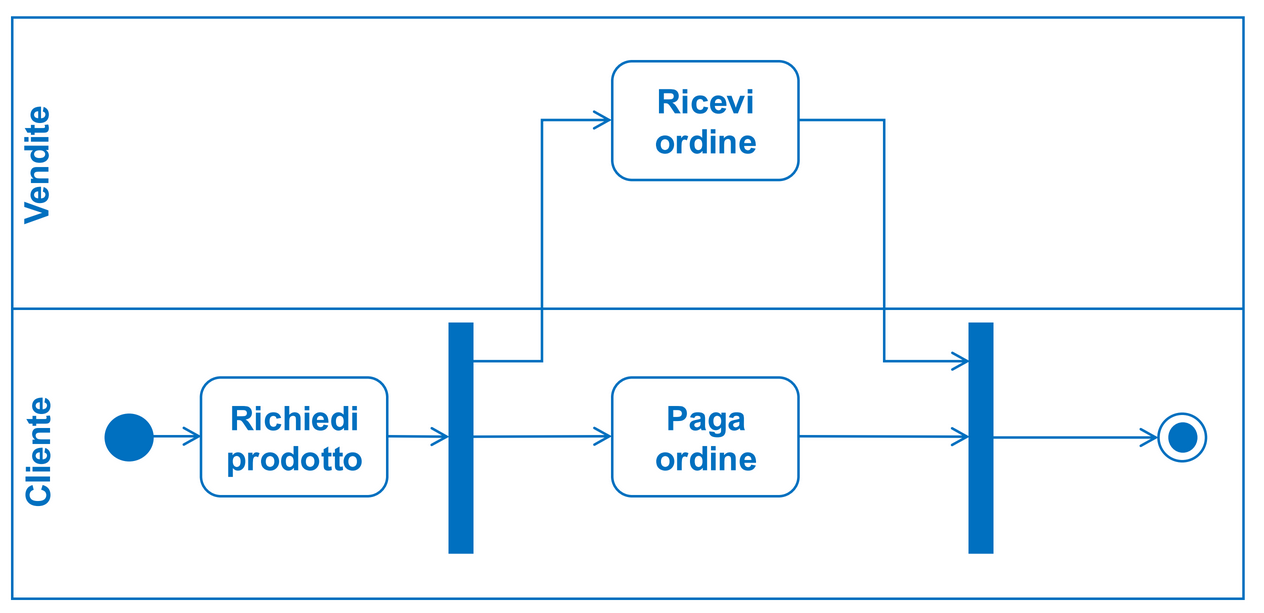
\includegraphics[scale=0.3]{partition.png}
\end{center}

\subsubsection{Diagramma degli stati}
Il comportamento di una classe viene descritto da un \textbf{grafo stati-transizioni}. Questo contiene gli \textbf{stati} significativi di un oggetto durante la sua vita e come questo può \textbf{transire} (in seguito ad eventi come messaggi) tra di essi.\\
Gli elementi principali sono lo stato \textbf{iniziale}, quello \textbf{finale}, gli stati \textbf{intermedi} e le \textbf{transizioni}. Queste ultime definiscono la risposta di un oggetto all'occorrenza di un evento e possono essere prese solo quando si verifica l'evento e l'eventuale \textbf{condizione} è vera. Comportano inoltre l'esecuzione di eventuali \textbf{azioni}.
\begin{center}
	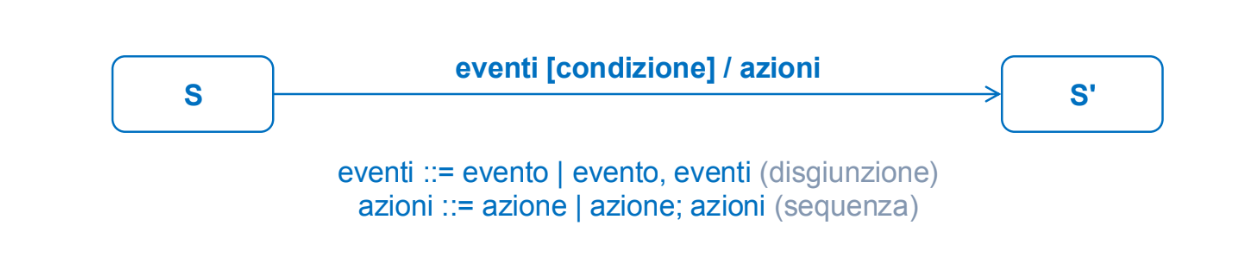
\includegraphics[scale=0.3]{transitions.png}
\end{center}

\begin{example}
	Un esempio di diagramma a stati con una classe \textit{Telefono} e un'operazione \textit{dial digit(n)}
	\begin{center}
		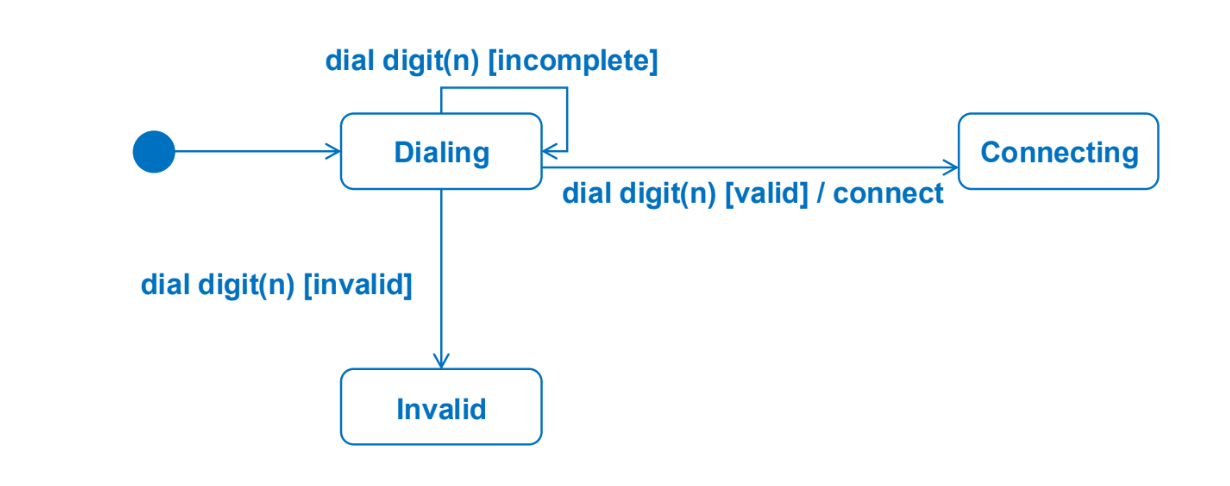
\includegraphics[scale=0.3]{state_machine.png}
	\end{center}
\end{example}

\paragraph{Eventi}
Un evento occorre \textbf{istantaneamente} e va introdotto solo se ha degli effetti. Se lo stato \textbf{non ha transizioni} per quell'evento, allora lo si ignora, altrimenti se ne ha \textbf{più di una}, si fa una scelta non-deterministica. Un evento può essere:
\begin{itemize}
	\item Un'\textbf{operazione} o un \textbf{segnale}: ricezione do una chiamata di metodo o un segnale con parametri e tipi compatibili
	\begin{equation*}
		op(a:T)
	\end{equation*}
	\item \textbf{Variazione}, quando \textit{exp} si verifica. Non avviene istantaneamente ma lo diventa appena si verifica l'espressione.
	\begin{equation*}
		when(exp)
	\end{equation*}
	\item \textbf{Temporale}, dopo che l'oggetto è stato fermo per un certo periodo di tempo
	\begin{equation*}
		after(t)
	\end{equation*}
\end{itemize}

\begin{example}
	Continuiamo l'esempio di prima aggiungendo due eventi di \textit{variazione}.
	\begin{center}
		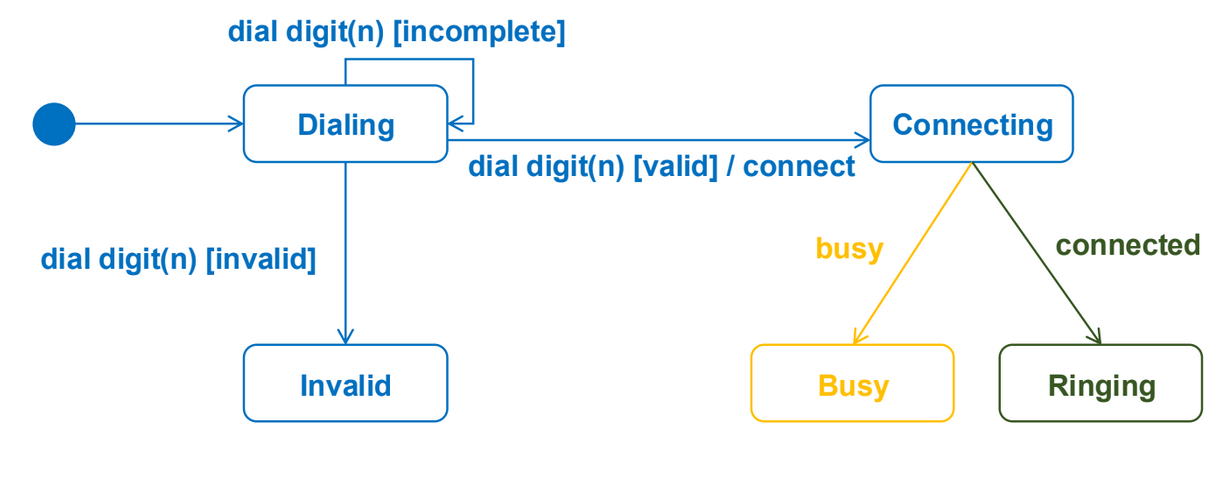
\includegraphics[scale=0.3]{variation.png}
	\end{center}
\end{example}

\paragraph{Stato}
Di seguito i comportamenti di un oggetto in determinate situazioni mentre esso si trova in un certo stato:
\begin{itemize}
	\item \textbf{entry}: azione di entrata eseguita all'ingresso in uno stato
	\item \textbf{do}: azione interna eseguita in modo continuativo mentre l'oggetto è in quello stato. Non necessita di eventi scatenanti, consuma tempo e può essere interrotta
	\item \textbf{exit}: azione di uscita eseguita all'ingresso in uno stato
	\item Eventuali \textbf{transizioni interne} che vengono eseguite in risposta ad un evento
\end{itemize}
\newpage
\begin{example}
	Prendiamo ad esempio lo stato di lettura di una password:
	\begin{center}
		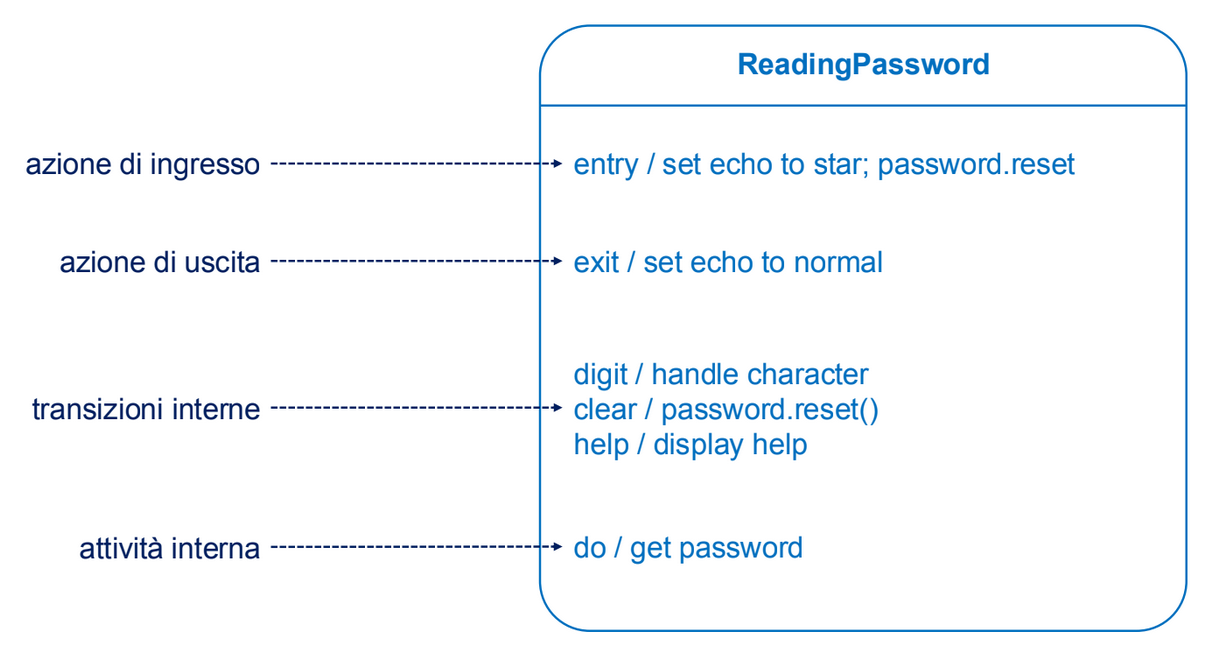
\includegraphics[scale=0.25]{reading_pw.png}
	\end{center}
\end{example}

\begin{note}
	I nomi degli stati devono indicarne la \textit{permanenza} e quindi dovrebbero essere aggettivi, participi passati o gerundi.
\end{note}

\paragraph{Stato composito}
In questo caso lo stato include un'ulteriore macchina a stati.\\
Il punto d'\textbf{ingresso} è determinato dalla freccia:
\begin{itemize}
	\item se arriva al bordo si inizia dallo stato iniziale della macchina interna
	\item altrimenti dallo stato indicato dalla freccia
\end{itemize}
 All'\textbf{uscita} ci possono essere tre casi:
 \begin{itemize}
 	\item Transizioni etichettate che partono dal bordo e possono essere attivate da qualsiasi stato interno
 	\item Dallo stato finale si procede alla \textbf{transizione di completamento}
 	\item Transizioni da stati interni che attraversano il bordo
 \end{itemize}
 
 \begin{center}
 	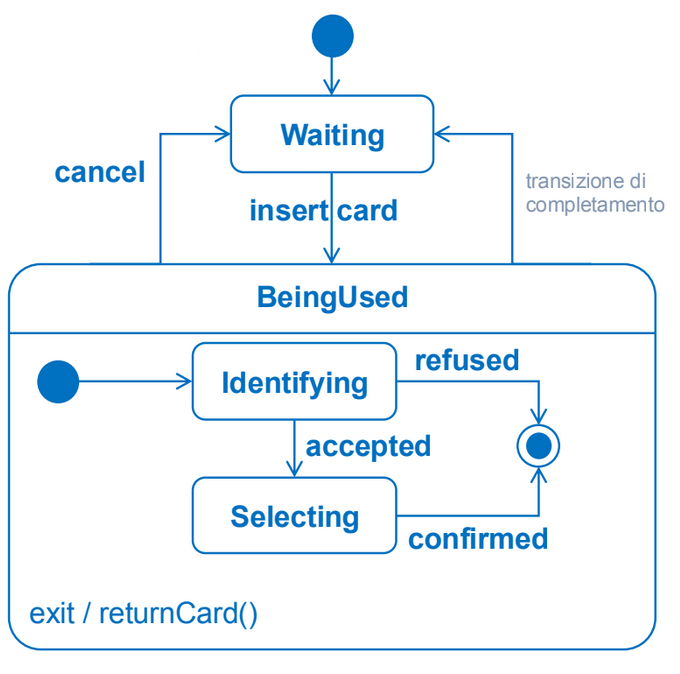
\includegraphics[scale=0.3]{stato_composito.png}
 \end{center}
 \newpage
 \paragraph{Stati compositi paralleli}
 È possibile avere stati compositi \textbf{paralleli}: possono esserci più sottostati attivi contemporaneamente, uno per regione. L'ingresso (\textbf{default entry}) arriva sul bordo e prosegue a tutti i sottostati iniziali. La transizione di uscita si può presentare in tre casi:
 \begin{itemize}
 	\item Transizione di completamento attivata al raggiungimento di tutti i sottostati finali
 	\item Transizione che esce da un solo sottostato e li termina tutti
 	\item Trasmissione che parte dal bordo, sempre attivabile e termina tutti i sottostati
 \end{itemize}
 
 \begin{center}
 	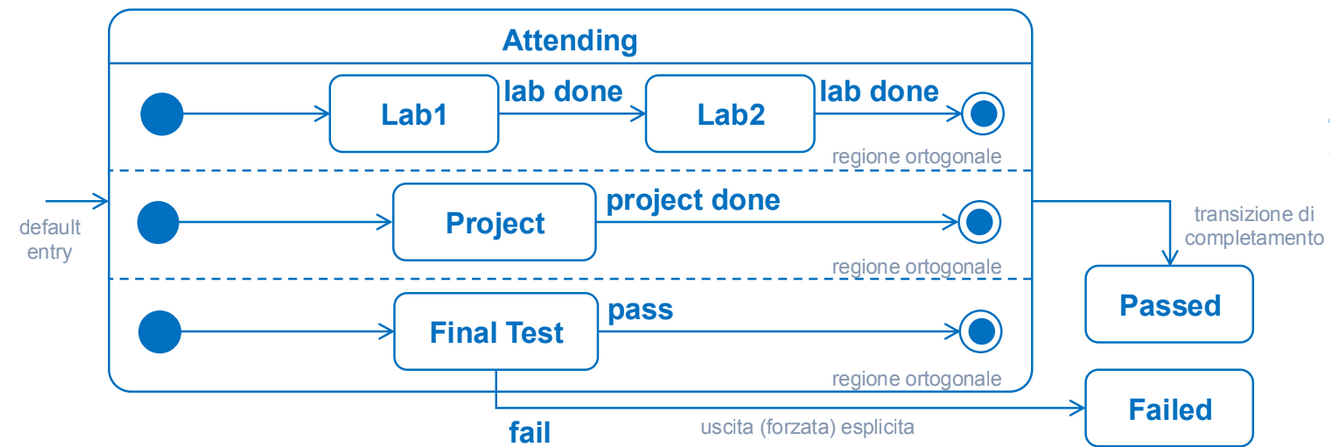
\includegraphics[scale=0.3]{stato_composito_parallelo.png}
 \end{center}
 
 \paragraph{Pseudo-stati}
 Esistono tre tipi di pseudo-stati:
 \begin{itemize}
 	\item \textbf{Scelta}: scelta basata su condizioni determinate \textbf{dinamicamente}. La disgiunzione (OR) di tutte le guardie deve essere sempre vera ed è ammesso il non-determinismo
 	\begin{center}
 		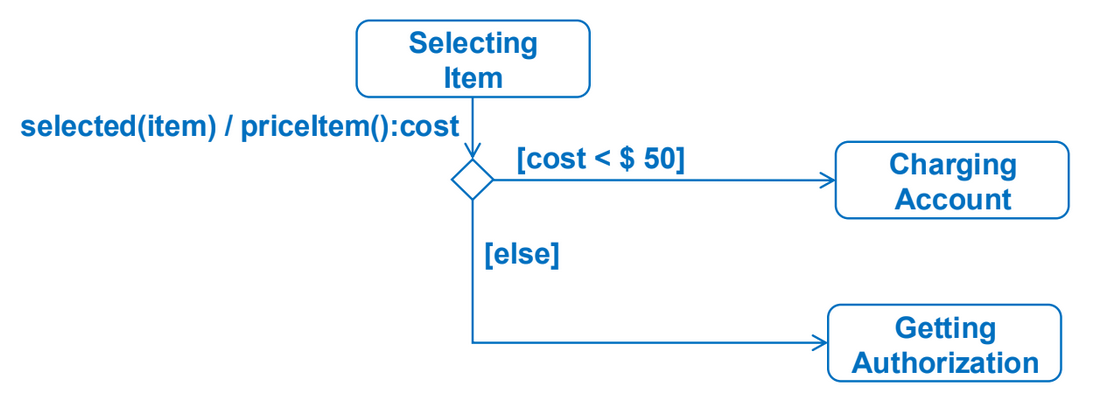
\includegraphics[scale=0.2]{choice.png}
 	\end{center}
 	\item \textbf{Giunzione}: pseudo-stato da cui escono e/o entrano due o più transizioni. Le condizioni sono valutate \textbf{staticamente} e \textbf{prima degli eventi} che attivano le transizioni in ingresso
 	\begin{center}
 		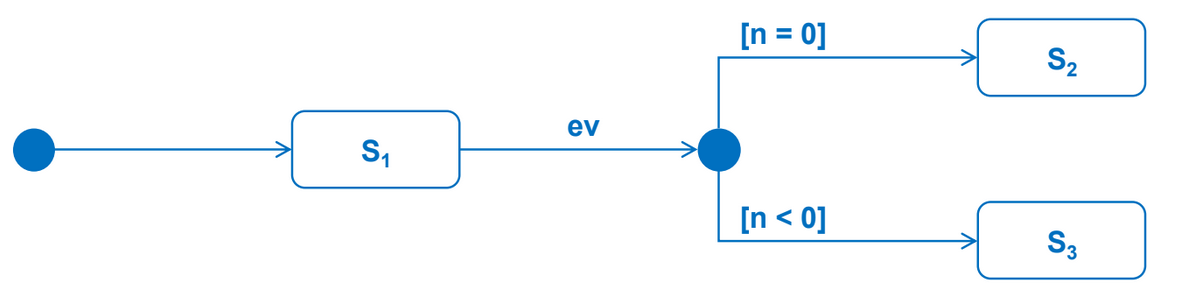
\includegraphics[scale=0.2]{giunzione.png}
 	\end{center}
 	\item \textbf{History}: permette di ripristinare lo stato della precedente attivazione dello stato composito
 	\begin{center}
 		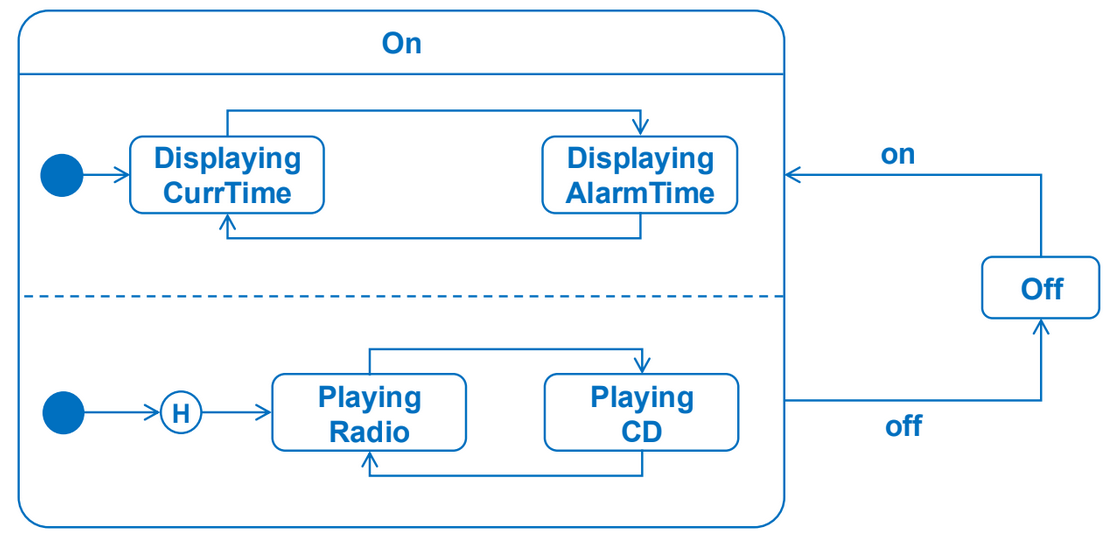
\includegraphics[scale=0.2]{history.png}
 	\end{center}
 \end{itemize}
 
 \paragraph{Sottomacchina}
 Una sottomacchina permette di descrivere uno stato composito in una macchina a parte. Ha un \textbf{nome} o \textbf{tipo} e le sue istanze sono nella forma
 \begin{equation*}
 	\text{nomeIstanza}:\text{Tipo}
 \end{equation*}
 Bisogna definire \textbf{entry} ed \textbf{exit} point per collegare la sottomacchina alle transizioni di quella principale. Le \textbf{transizioni di completamento} scattano quando:
 \begin{itemize}
 	\item Si raggiunge la \textbf{terminazione}:
 	\begin{itemize}
 		\item Stato finale per lo \textit{stato composito sequenziale}
 		\item Stati finali di tutte le regioni ortogonali per lo \textit{stato composito parallelo}
 		\item Exit point
 	\end{itemize}
 	\item Alla terminazione di \textbf{entry} e/o \textbf{do}
 	\item Al raggiungimento di uno pseudo-stato \textbf{giunzione}
 \end{itemize}
 \begin{center}
 	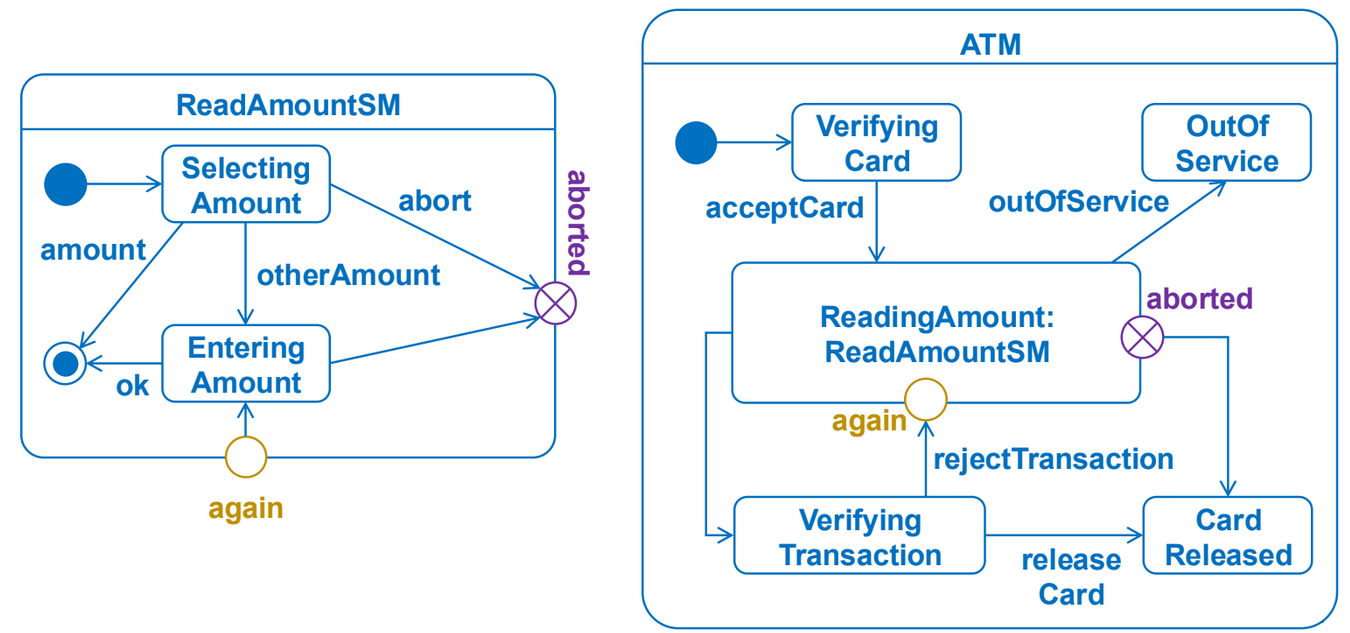
\includegraphics[scale=0.3]{sottomacchina.png}
 \end{center}
 \begin{note}
 	L'attività \textbf{exit} viene eseguita quando scatta la transizione di completamento.
 \end{note}
 
 \begin{observation}[Attività vs stati]
 	Il diagramma degli stati serve a mostrare l'evoluzione di un oggetto in risposta a degli eventi e descrive quindi l'evoluzione delle istanze. Quello delle attività, invece, permette di mettere in ordine le attività da fare descrivendo il flusso delle azioni da svolgere.
 \end{observation}